\documentclass[tikz]{standalone}
\usetikzlibrary{calc,arrows,math}

\begin{document}
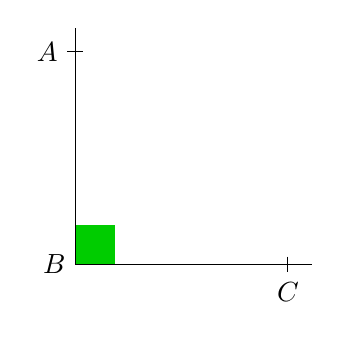
\begin{tikzpicture}
    \tikzmath{ \r=90; }
    \coordinate (B) at (0,0);
    \coordinate (A) at ({3*cos(\r)},{3*sin(\r)});
    \coordinate (C) at (3,0);
    \fill[green!80!black] (B) rectangle +(0.5,0.5);
    \draw (A) -- (B) -- (C);
    \draw ($(B)!0.9!(A) + (-0.1,0)$) node[left]{$A$} -- ++(0.2,0);
    \draw ($(B)!0.9!(C) + (0,0.1)$) -- ++(0,-0.2) node[below]{$C$};
    \node[left] at (B) {$B$};
\end{tikzpicture}
\end{document}